\documentclass[10pt,a4paper]{article}

\usepackage[spanish,activeacute,es-tabla]{babel}
\usepackage[utf8]{inputenc}
\usepackage{ifthen}
\usepackage{listings}
\usepackage{dsfont}
\usepackage{subcaption}
\usepackage{amsmath}
\usepackage[strict]{changepage}
\usepackage[top=1cm,bottom=2cm,left=1cm,right=1cm]{geometry}%
\usepackage{color}%
\newcommand{\tocarEspacios}{%
	\addtolength{\leftskip}{3em}%
	\setlength{\parindent}{0em}%
}

% Especificacion de procs

\newcommand{\In}{\textsf{in }}
\newcommand{\Out}{\textsf{out }}
\newcommand{\Inout}{\textsf{inout }}

\newcommand{\encabezadoDeProc}[4]{%
	% Ponemos la palabrita problema en tt
	%  \noindent%
	{\normalfont\bfseries\ttfamily proc}%
	% Ponemos el nombre del problema
	\ %
	{\normalfont\ttfamily #2}%
	\
	% Ponemos los parametros
	(#3)%
	\ifthenelse{\equal{#4}{}}{}{%
		% Por ultimo, va el tipo del resultado
		\ : #4}
}

\newenvironment{proc}[4][res]{%
	
	% El parametro 1 (opcional) es el nombre del resultado
	% El parametro 2 es el nombre del problema
	% El parametro 3 son los parametros
	% El parametro 4 es el tipo del resultado
	% Preambulo del ambiente problema
	% Tenemos que definir los comandos requiere, asegura, modifica y aux
	\newcommand{\requiere}[2][]{%
		{\normalfont\bfseries\ttfamily requiere}%
		\ifthenelse{\equal{##1}{}}{}{\ {\normalfont\ttfamily ##1} :}\ %
		\{\ensuremath{##2}\}%
		{\normalfont\bfseries\,\par}%
	}
	\newcommand{\asegura}[2][]{%
		{\normalfont\bfseries\ttfamily asegura}%
		\ifthenelse{\equal{##1}{}}{}{\ {\normalfont\ttfamily ##1} :}\
		\{\ensuremath{##2}\}%
		{\normalfont\bfseries\,\par}%
	}
	\renewcommand{\aux}[4]{%
		{\normalfont\bfseries\ttfamily aux\ }%
		{\normalfont\ttfamily ##1}%
		\ifthenelse{\equal{##2}{}}{}{\ (##2)}\ : ##3\, = \ensuremath{##4}%
		{\normalfont\bfseries\,;\par}%
	}
	\renewcommand{\pred}[3]{%
		{\normalfont\bfseries\ttfamily pred }%
		{\normalfont\ttfamily ##1}%
		\ifthenelse{\equal{##2}{}}{}{\ (##2) }%
		\{%
		\begin{adjustwidth}{+5em}{}
			\ensuremath{##3}
		\end{adjustwidth}
		\}%
		{\normalfont\bfseries\,\par}%
	}
	
	\newcommand{\res}{#1}
	\vspace{1ex}
	\noindent
	\encabezadoDeProc{#1}{#2}{#3}{#4}
	% Abrimos la llave
	\par%
	\tocarEspacios
}
{
	% Cerramos la llave
	\vspace{1ex}
}

\newcommand{\aux}[4]{%
	{\normalfont\bfseries\ttfamily\noindent aux\ }%
	{\normalfont\ttfamily #1}%
	\ifthenelse{\equal{#2}{}}{}{\ (#2)}\ : #3\, = \ensuremath{#4}%
	{\normalfont\bfseries\,;\par}%
}

\newcommand{\pred}[3]{%
	{\normalfont\bfseries\ttfamily\noindent pred }%
	{\normalfont\ttfamily #1}%
	\ifthenelse{\equal{#2}{}}{}{\ (#2) }%
	\{%
	\begin{adjustwidth}{+2em}{}
		\ensuremath{#3}
	\end{adjustwidth}
	\}%
	{\normalfont\bfseries\,\par}%
}

% Tipos

\newcommand{\nat}{\ensuremath{\mathds{N}}}
\newcommand{\ent}{\ensuremath{\mathds{Z}}}
\newcommand{\float}{\ensuremath{\mathds{R}}}
\newcommand{\bool}{\ensuremath{\mathsf{Bool}}}
\newcommand{\cha}{\ensuremath{\mathsf{Char}}}
\newcommand{\str}{\ensuremath{\mathsf{String}}}

% Logica

\newcommand{\True}{\ensuremath{\mathrm{true}}}
\newcommand{\False}{\ensuremath{\mathrm{false}}}
\newcommand{\Then}{\ensuremath{\rightarrow}}
\newcommand{\Iff}{\ensuremath{\leftrightarrow}}
\newcommand{\implica}{\ensuremath{\longrightarrow}}
\newcommand{\IfThenElse}[3]{\ensuremath{\mathsf{if}\ #1\ \mathsf{then}\ #2\ \mathsf{else}\ #3\ \mathsf{fi}}}
\newcommand{\yLuego}{\land _L}
\newcommand{\oLuego}{\lor _L}
\newcommand{\implicaLuego}{\implica _L}

\newcommand{\cuantificador}[5]{%
	\ensuremath{(#2 #3: #4)\ (%
		\ifthenelse{\equal{#1}{unalinea}}{
			#5
		}{
			$ % exiting math mode
			\begin{adjustwidth}{+2em}{}
				$#5$%
			\end{adjustwidth}%
			$ % entering math mode
		}
		)}
}

\newcommand{\existe}[4][]{%
	\cuantificador{#1}{\exists}{#2}{#3}{#4}
}
\newcommand{\paraTodo}[4][]{%
	\cuantificador{#1}{\forall}{#2}{#3}{#4}
}

%listas

\newcommand{\TLista}[1]{\ensuremath{seq \langle #1\rangle}}
\newcommand{\lvacia}{\ensuremath{[\ ]}}
\newcommand{\lv}{\ensuremath{[\ ]}}
\newcommand{\longitud}[1]{\ensuremath{|#1|}}
\newcommand{\cons}[1]{\ensuremath{\mathsf{addFirst}}(#1)}
\newcommand{\indice}[1]{\ensuremath{\mathsf{indice}}(#1)}
\newcommand{\conc}[1]{\ensuremath{\mathsf{concat}}(#1)}
\newcommand{\cab}[1]{\ensuremath{\mathsf{head}}(#1)}
\newcommand{\cola}[1]{\ensuremath{\mathsf{tail}}(#1)}
\newcommand{\sub}[1]{\ensuremath{\mathsf{subseq}}(#1)}
\newcommand{\en}[1]{\ensuremath{\mathsf{en}}(#1)}
\newcommand{\cuenta}[2]{\mathsf{cuenta}\ensuremath{(#1, #2)}}
\newcommand{\suma}[1]{\mathsf{suma}(#1)}
\newcommand{\twodots}{\ensuremath{\mathrm{..}}}
\newcommand{\masmas}{\ensuremath{++}}
\newcommand{\matriz}[1]{\TLista{\TLista{#1}}}
\newcommand{\seqchar}{\TLista{\cha}}

\renewcommand{\lstlistingname}{Código}
\lstset{% general command to set parameter(s)
	language=Java,
	morekeywords={endif, endwhile, skip},
	basewidth={0.47em,0.40em},
	columns=fixed, fontadjust, resetmargins, xrightmargin=5pt, xleftmargin=15pt,
	flexiblecolumns=false, tabsize=4, breaklines, breakatwhitespace=false, extendedchars=true,
	numbers=left, numberstyle=\tiny, stepnumber=1, numbersep=9pt,
	frame=l, framesep=3pt,
	captionpos=b,
}

\usepackage{caratula} % Version modificada para usar las macros de algo1 de ~> https://github.com/bcardiff/dc-tex


\titulo{Trabajo Práctico 2}
\subtitulo{Clasificación y Selección de Modelos}

\fecha{\today}

\materia{Laboratorio de Datos}
\grupo{Grupo 100}

\integrante{Apellido, Nombre1}{001/01}{email1@dominio.com}
\integrante{Martinelli, Lorenzo}{364/23}{martinelli.lorenzo12@gmail.com}
\integrante{Padilla, Ramiro}{1636/21}{ramiromdq123@gmail.com}
% Pongan cuantos integrantes quieran

% Declaramos donde van a estar las figuras
% No es obligatorio, pero suele ser comodo
\graphicspath{{../static/}}

\begin{document}

\maketitle

\section{Introducción}  \vspace{0.1cm}

\subsection{Fuente de datos} \vspace{0.2cm}

A lo largo de este proyecto, trabajaremos con un conjunto de datos de imágenes denominado Sign
Language MNIST\footnote{Link al dataset https://www.kaggle.com/datasets/datamunge/sign-language-mnist}, el cual se encuentra en formato csv, donde cada imagen del set de datos representa una letra en lenguaje de señas americano. El link al dataset se encuentra al pie de página.

\subsection{Análisis exploratorio de datos}  \vspace{0.2cm}

Antes de ponernos a trabajar con los datos, necesitamos saber mas acerca de ellos. Sabemos que, cada fila del dataset representa una imagen de 28x28 pixeles en escala de grises que corresponde a una letra en lenguaje de señas. Miremos a continuación un pequeño fragmento del mismo. En este, podremos ver las semejanzas y diferencias que tenemos entre las distintas letras. También, se puede ver en menor medida similitudes entre letras de la misma clase.

 \vspace{0.2cm}

\begin{figure}[h]
  \centering
  \includegraphics[width=1.0\textwidth]{Imagenes/atributos\_relevantes.png}
  \caption{Primeras nueve imagenes del dataset}
  \label{fig:Tabla 1}
\end{figure}

 \vspace{0.2cm}

A partir del gráfico anterior, podemos inferir que no todos los pixeles son realmente relevantes para diferenciar imágenes entre si. Por ejemplo, podemos ver
que aquellos pixeles correspondientes al fondo no aportan información alguna. ¿Cuántos pixeles necesitaremos realmente para diferenciar las imágenes? \vspace{0.05cm}

Por otro lado, viendo por ejemplo, que las letras C y D aparecen más de una vez, también surge la pregunta. ¿Están balanceadas las distintas clases que identifican a las letras? En el gráfico a continuación, podremos notar que tenemos un dataset con una excelente distribución de clases. ¿Por qué me interesa
tener una cantidad pareja de cada muestra? Esto, adquiere relevancia puesto que al entrenar nuestros modelos en un futuro, no queremos tener sesgos.
\vspace{0.05cm}
  
Obs: Las letras J y Z no poseen ningún ejemplar puesto que requieren de movimiento para su seña.

\vspace{0.1cm}

\begin{figure}[h]
  \centering
  \includegraphics[width=0.8\textwidth]{Imagenes/distribucion.png}
  \caption{Cantidad de muestras de cada letra}
  \label{fig:Tabla 1}
\end{figure}

\newpage

Otra pregunta que naturalmente surge al explorar el dataser es que tan distintas son las letras entre sí, y si las diferentes muestras respecto a una misma letras
presentan diferencias notorias o no. Para eso, comparemos por ejemplo, las letras E, L y M.

\begin{figure}[ht!]
	\begin{subfigure}{0.5\textwidth}
		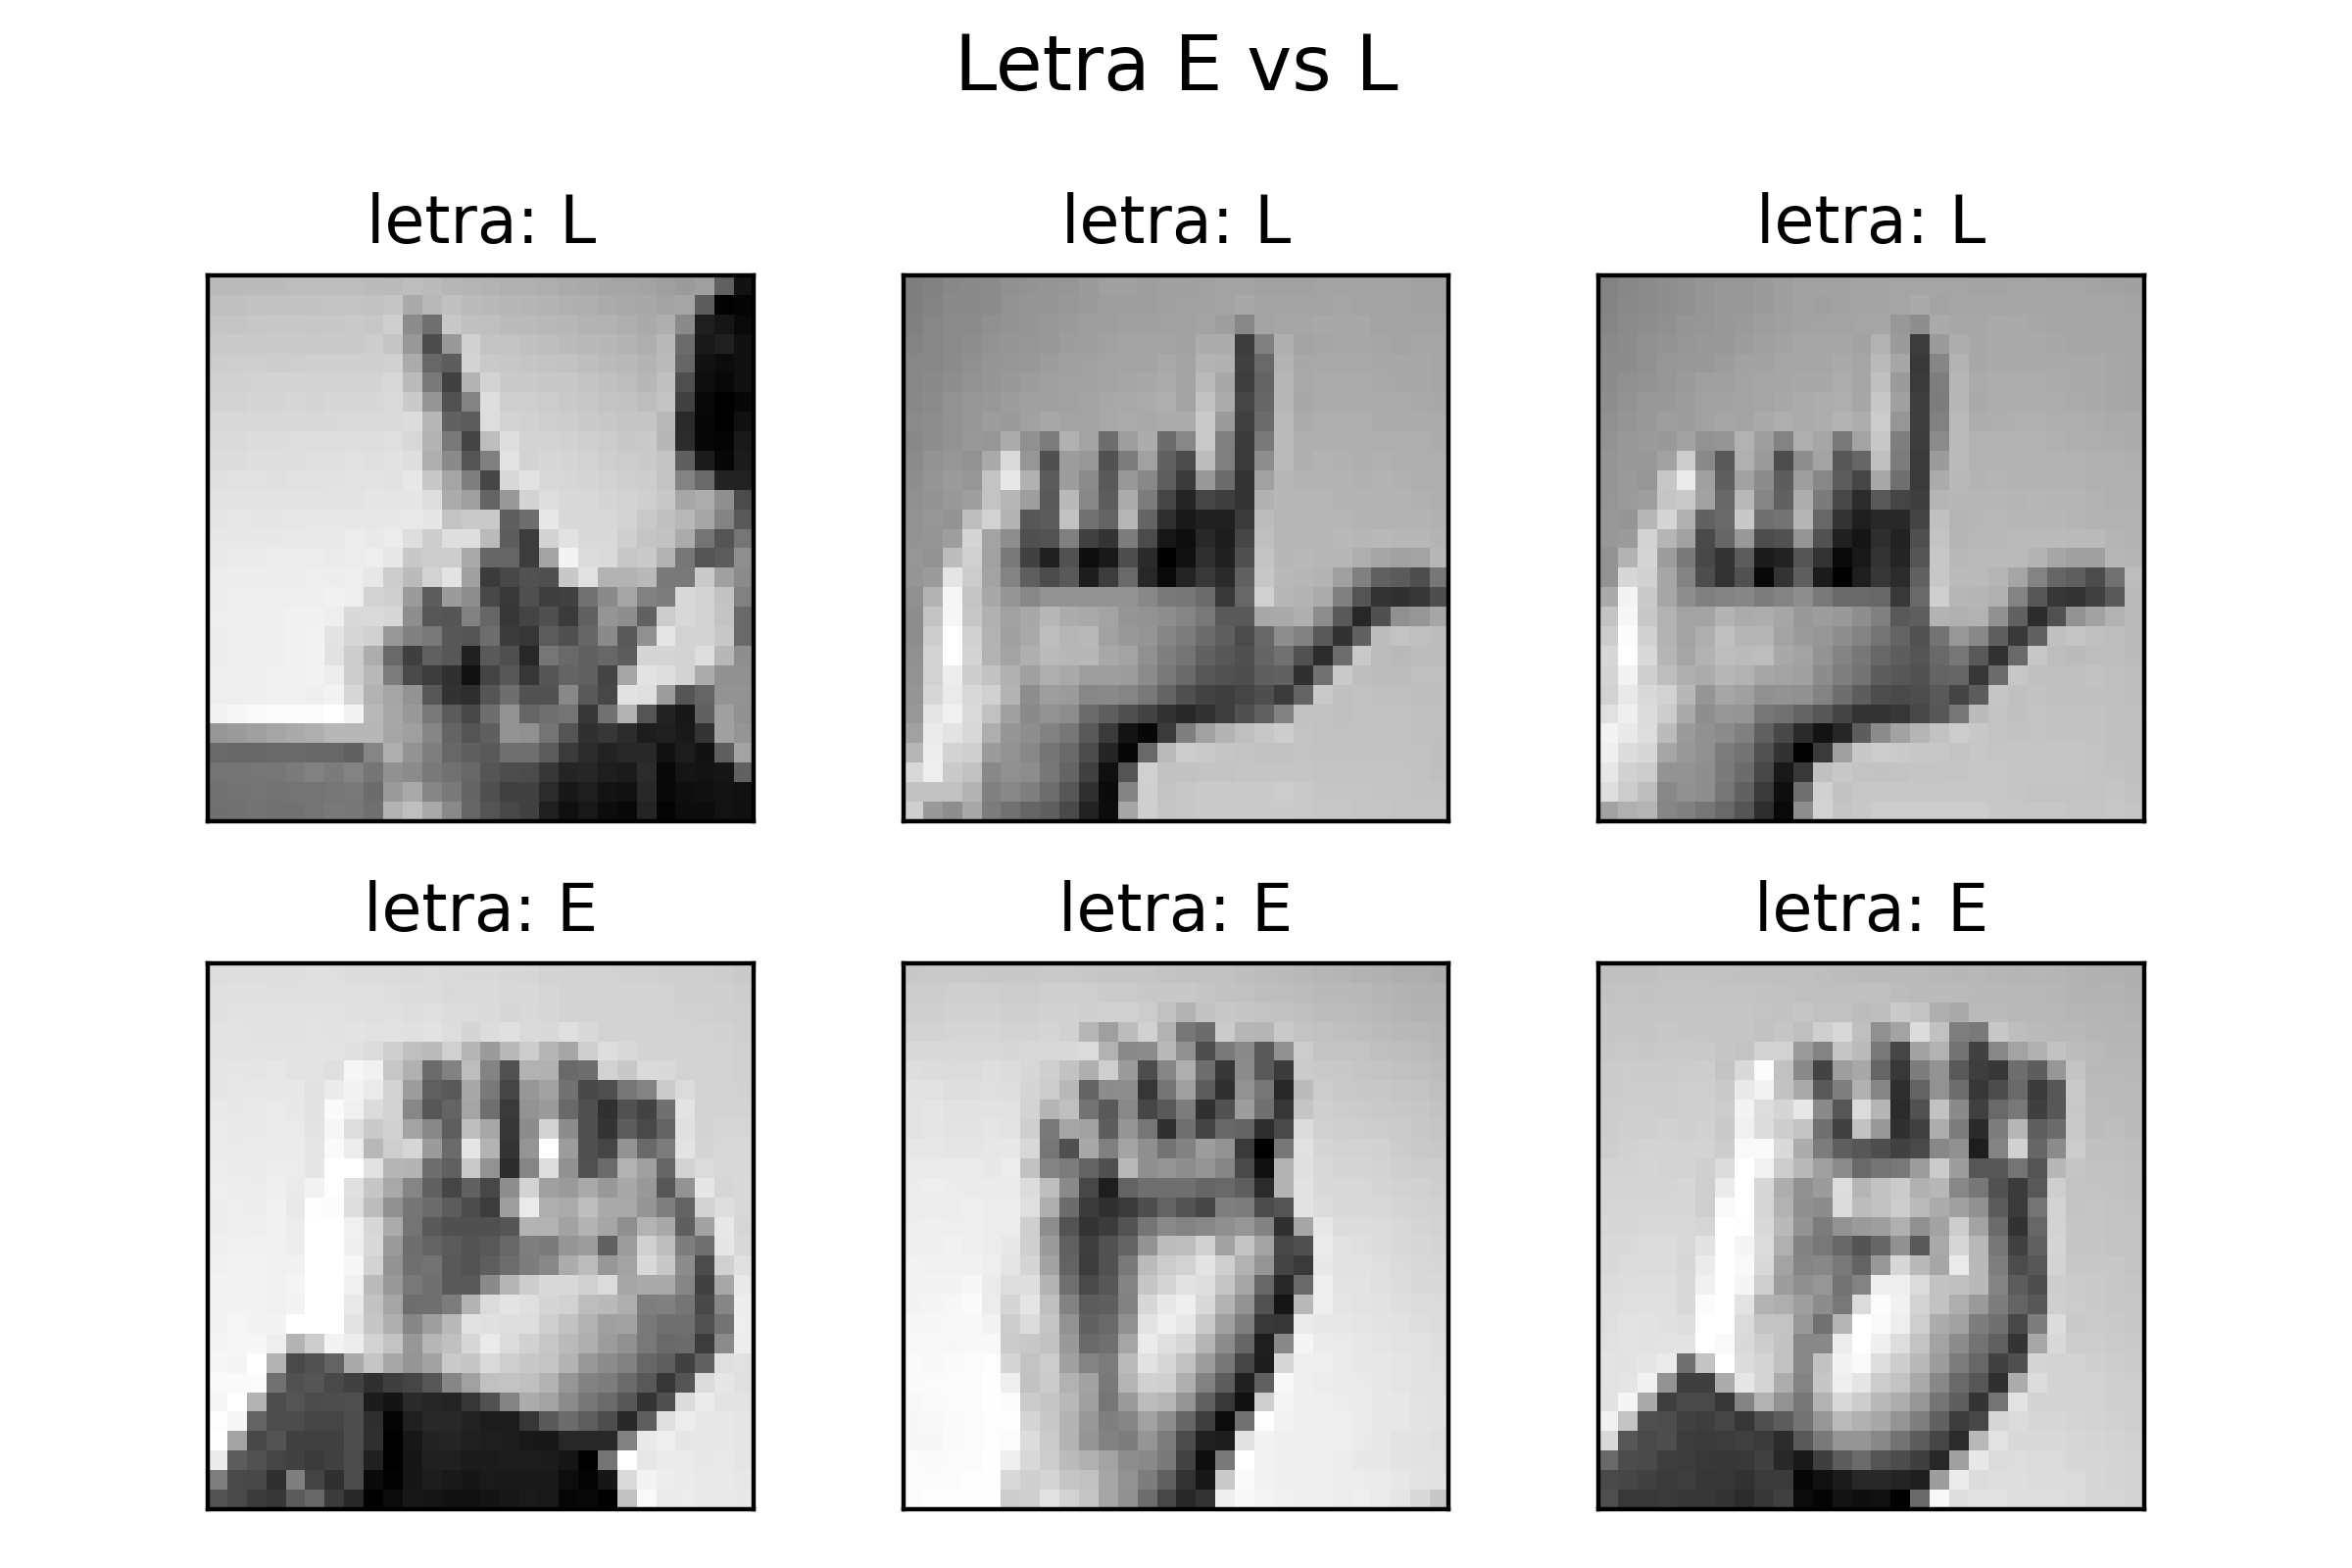
\includegraphics[width=0.9\linewidth]{Imagenes/letra_E_vs_L.png} 
		\caption{Muestras de las letras E y L}
		\label{fig:subfig1}
	\end{subfigure}
	\begin{subfigure}{0.5\textwidth}
		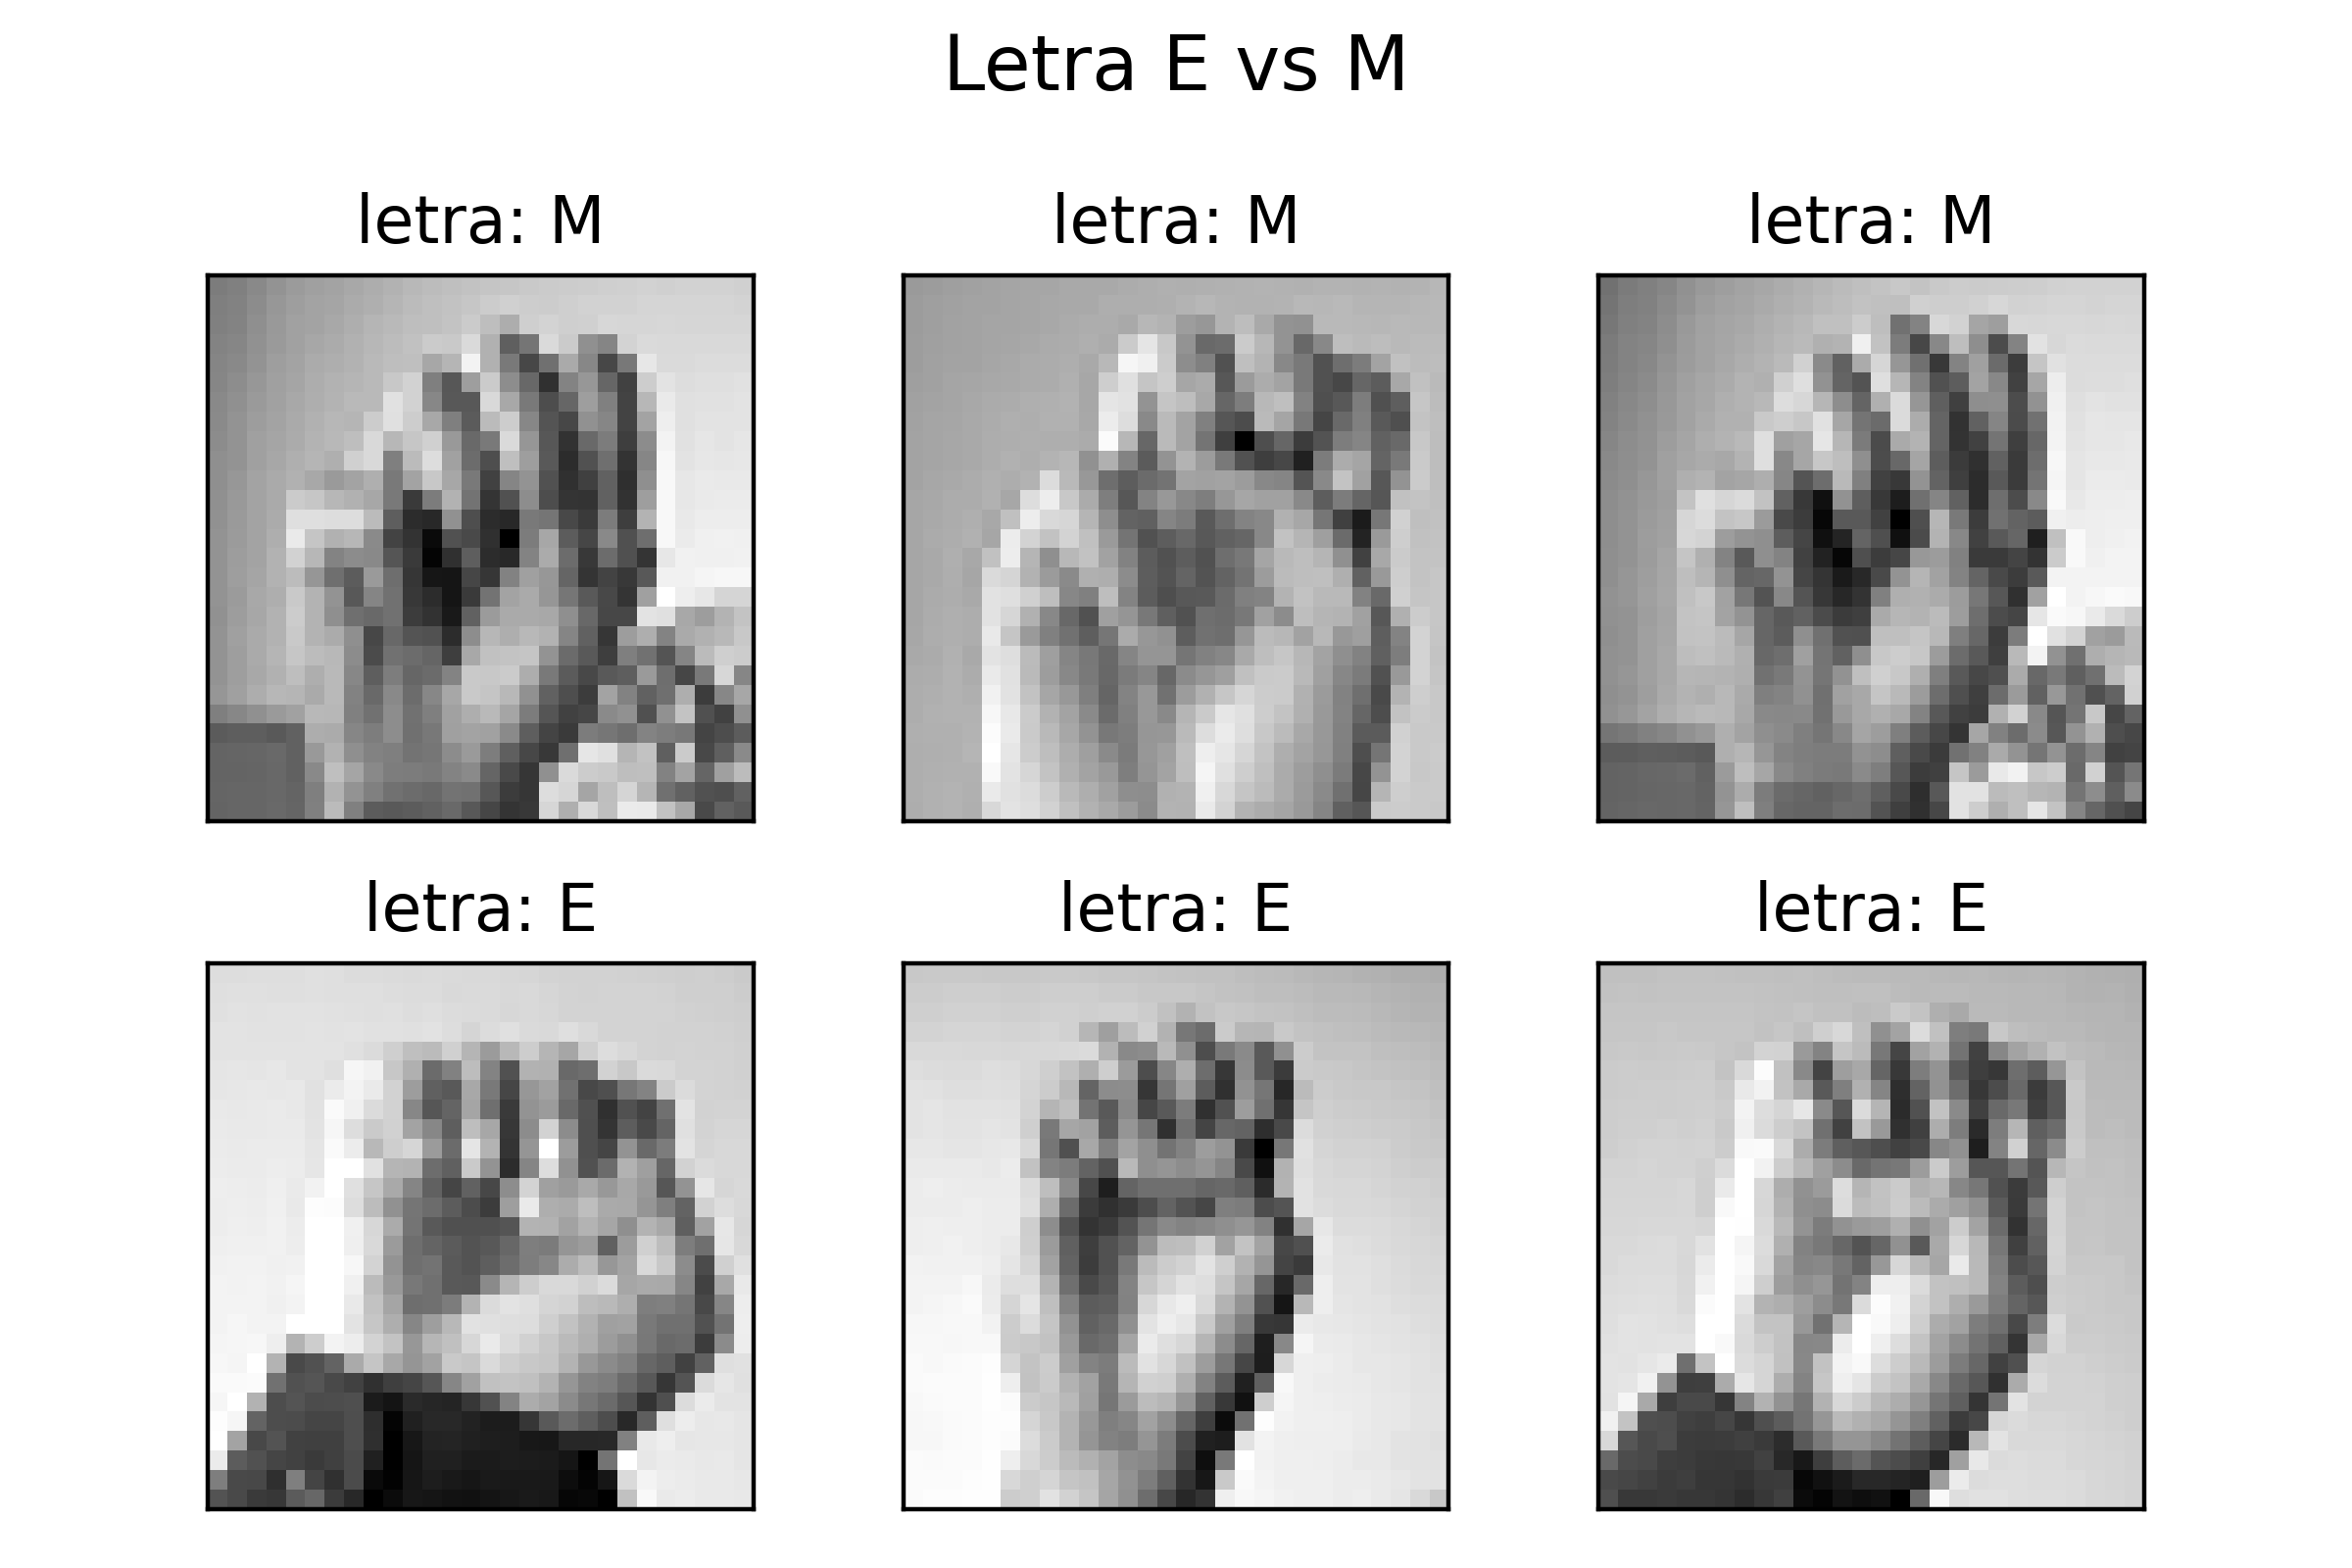
\includegraphics[width=0.9\linewidth]{Imagenes/letra_E_vs_M.png}
		\caption{Muestras de las letras E y M}
		\label{fig:subfig2}
	\end{subfigure}
	% OJO: el caption siempre va antes del label
	\label{fig:subfigs}
\end{figure}

En la imagen anterior, podemos apreciar que tanto la letra E como la M son muy distintas a la letra L, sin embargo, poseen muchas semenjanzas entre sí. Esto, es algo a tener en cuenta a la hora de plantear los modelos, cuales serán los pixeles mas representativos para imagenes similares.
Miremos también, si en imagenes pertenencientes a una misma letra hay diferencias notorias. 

\begin{figure}[ht!]
	\begin{subfigure}{0.5\textwidth}
		\centering
		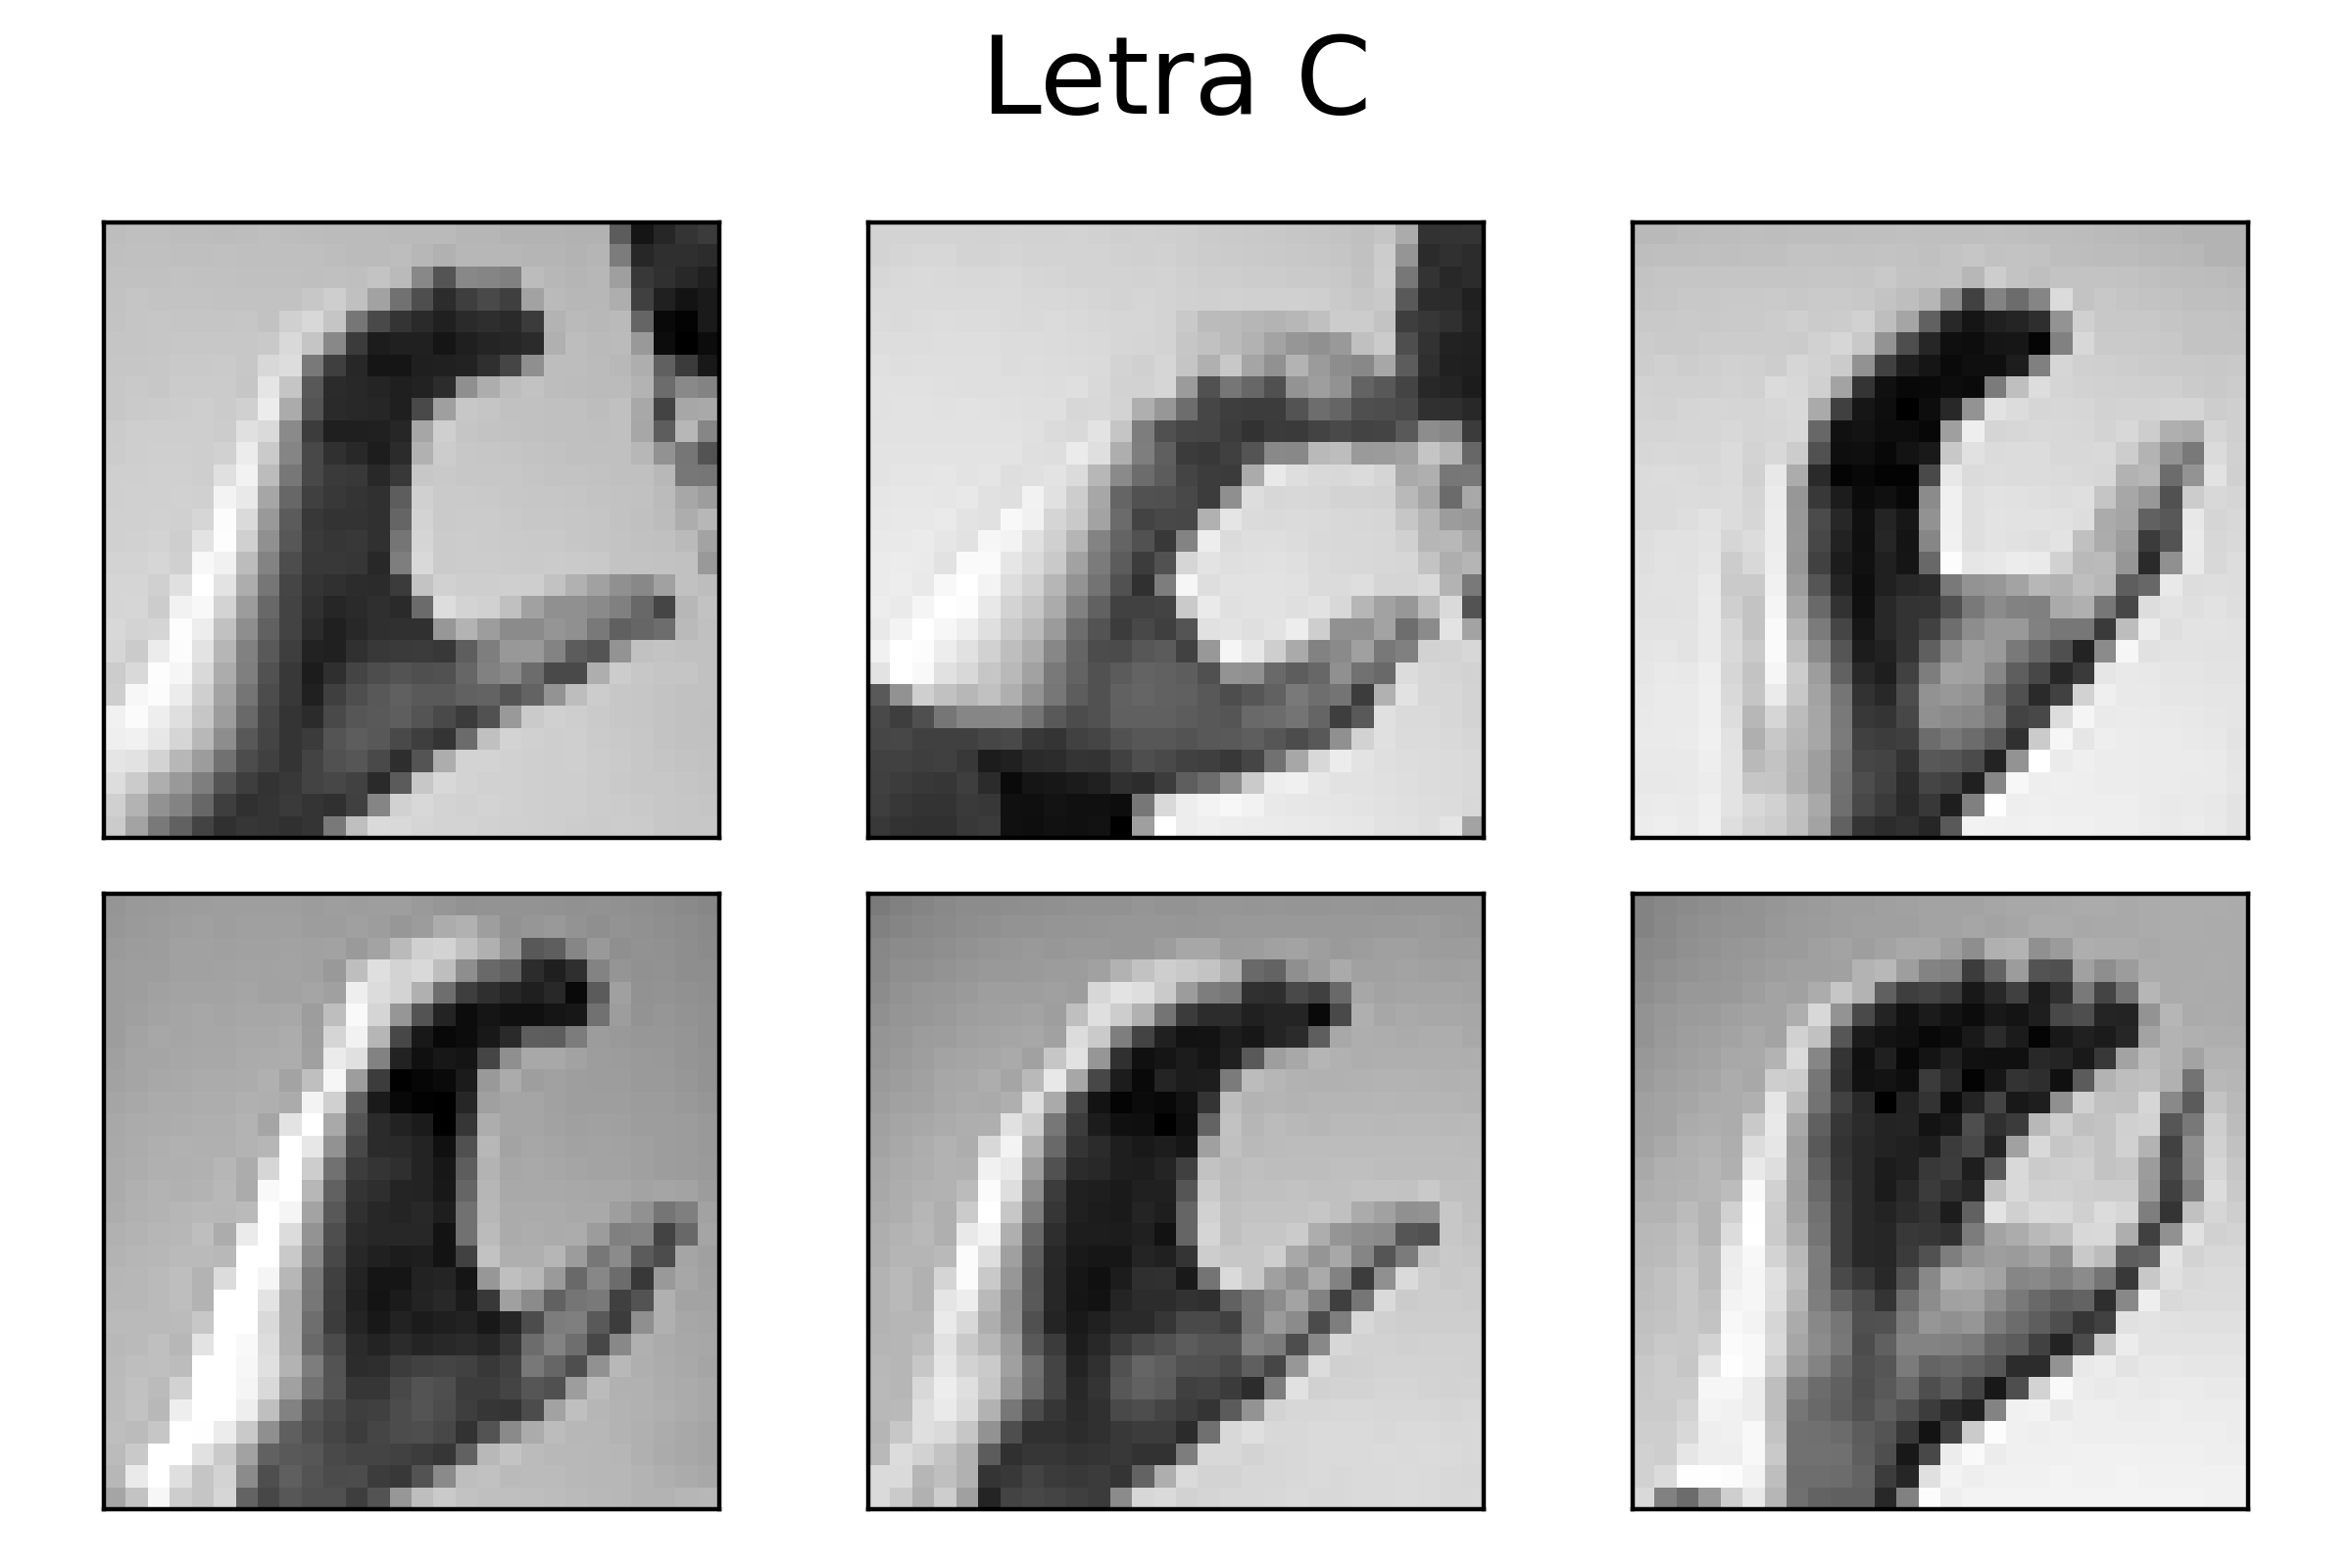
\includegraphics[width=1\linewidth]{Imagenes/letra_C.png} 
		\caption{Distintas muestras de la letra C}
		\label{fig:subfig1}
	\end{subfigure}
	\begin{subfigure}{0.55\textwidth}
		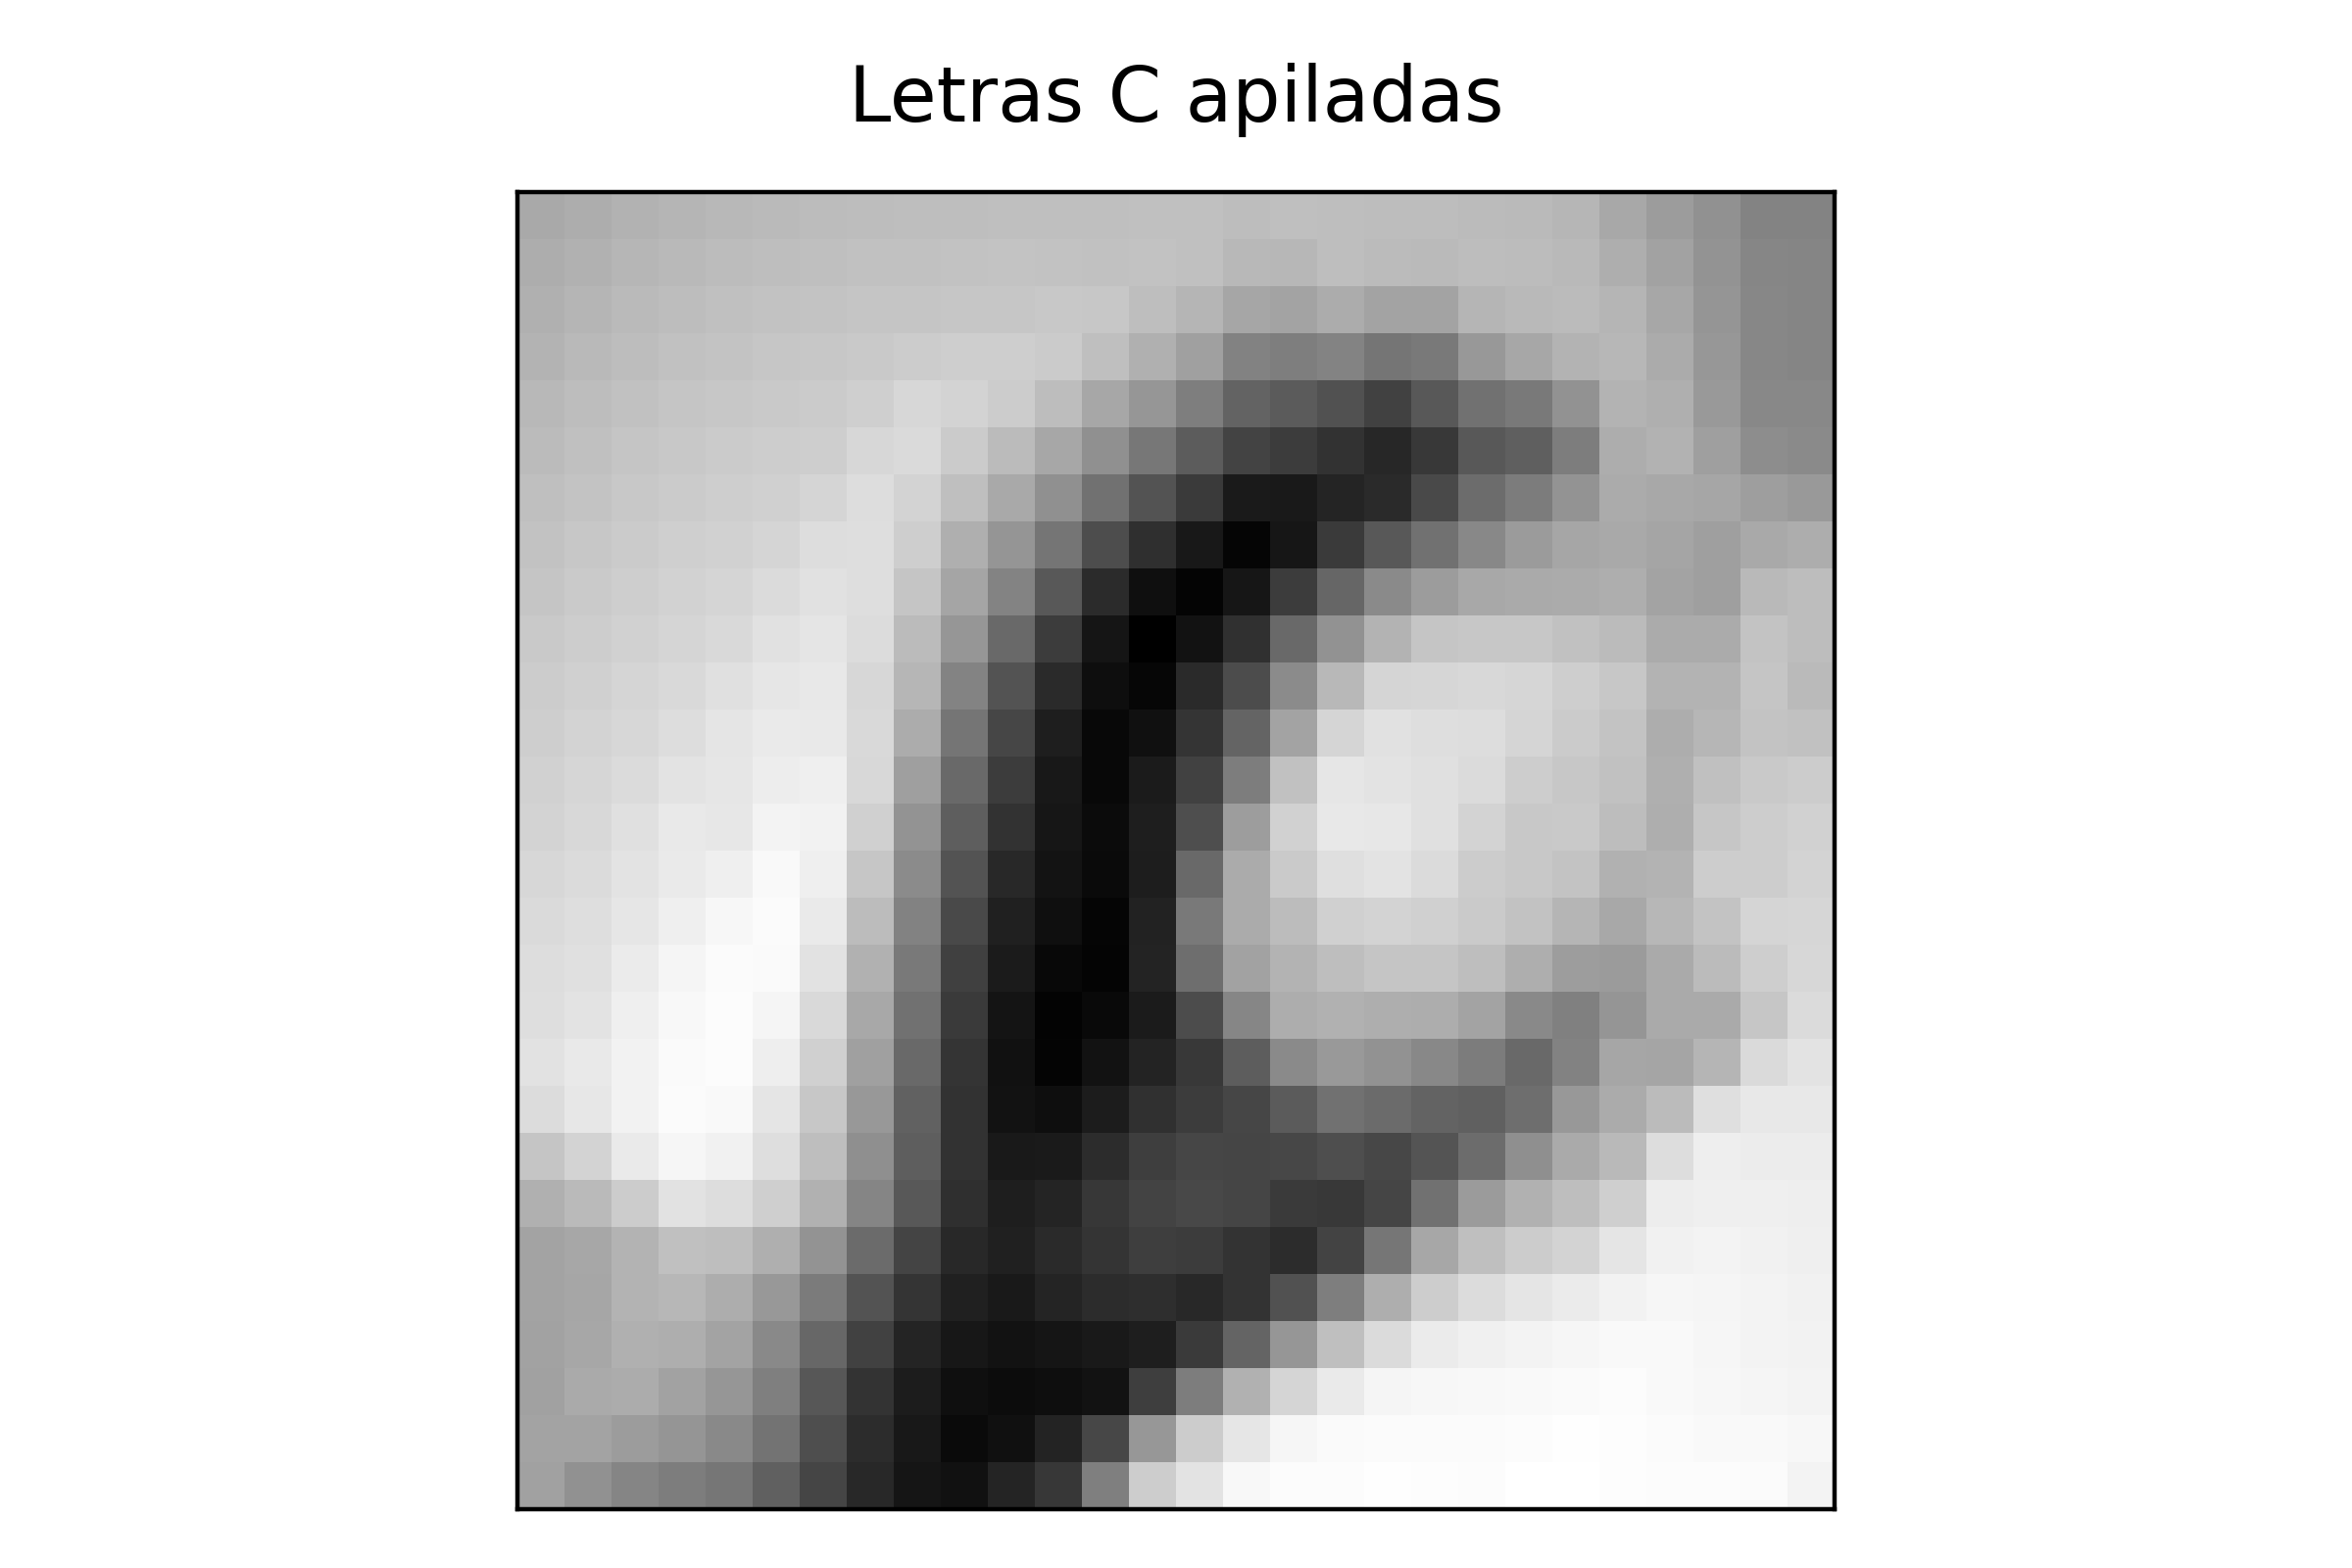
\includegraphics[width=1\linewidth]{Imagenes/letra_C_apilada.png}
		\caption{Todas las muestras de la letra C apiladas}
		\label{fig:subfig2}
	\end{subfigure}
	% OJO: el caption siempre va antes del label
	\label{fig:subfigs}
\end{figure}

\newpage

Si bien, a simple vista, cuando comparamos algunos ejemplares, pareciera que las diferencias pueden llegar a ser significativas, a la hora de comparar todos los ejemplares, en este caso, apilandolos, notamos que forman una silueta que representa muy bien la seña a la que corresponde. \vspace{0.1cm}

A partir de todo el análisis anterior, pudimos notar que no representa diferencias significativas el trabajar con imagenes respecto a datasets como el del titanic, respecto a su dificultad. Si, quizas, lleva algo mas de tiempo su análisis, pero con las herramientas indicadas no presenta mayores dificultades.

\vspace{0.1cm}


\section{Modelo}

\subsection{¿La imagen corresponde a una seña de la L o a una seña de la A?} \vspace{0.1cm}

En esta sección, trabajeremos con un subconjunto del dataset original, donde solo esten la letra A  y L. Nuestro objetivo, será encontrar un modelo que
diferencie con la menor cantidad de pixeles posibles. Comencemos entonces, viendo las diferencias entre estas letras y cuantas muestras tenemos. 

\begin{figure}[ht!]
	\begin{subfigure}{0.5\textwidth}
		\centering
		\includegraphics[width=1\linewidth]{Imagenes/letras\_A\_L\_apiladas.png} 
		\caption{Todas las letras A y L apiladas y reescaladas}
		\label{fig:subfig1}
	\end{subfigure}
	\begin{subfigure}{0.55\textwidth}
		\includegraphics[width=1\linewidth]{Imagenes/cantidad\_letras\_A\_L.png}
		\caption{Cantidad por clase}
		\label{fig:subfig2}
	\end{subfigure}
	% OJO: el caption siempre va antes del label
	\label{fig:subfigs}
\end{figure}

Sabemos entonces, que tenemos buena distribución, y podemos ver de la imagen de la izquierda que pareceria que hay dos zonas que diferencian bien ambas letras, lo que vamos a hacer entonces es 'restar' ambas letras para asi encontrar donde estan los pixeles de mayor varianza. ¿Por qué los de mayor varianza? Puesto que son aquellos que representan mas la diferencia entre ambas imagenes. 

\begin{figure}[h]
  \centering
  \includegraphics[width=0.8\textwidth]{Imagenes/varianza.png}
  \caption{Letra L - A}
  \label{fig:Tabla 1}
\end{figure}

Notamos que, la zona con mayor varianza seria en la zona mas oscura que aparece en el medio de la imagen o, en su defecto, la zona mas blanca. Para saber esto con precisión utilizamos una función de pandas que nos devuelve en una lista las 10 posiciones con los valores mas altos. Destacando, que los pixeles
mas representativos son el 301, 274 y 246. 

\subsection{Construcción del Modelo} \vspace{0.1cm}

Una vez, que conocemos bastante acerca de nuestro dataset, estamos en condiciones de armar nuestro clasificador Knn. A fines de afinar nuestro modelo, hicimos pruebas utilizando distintas cantidades de pixeles, la idea es, utilizar la menor cantidad posible para asi no usar datasets tan grandes. \vspace{0.05cm}
Como ya conociamos aquellos pixeles mas significativos, hicimos pruebas utilizando 1, 3 y 50 pixeles tomando a su vez, distinta cantidad de vecinos. 
A continuación tenemos los resultados.

\begin{figure}[ht!]
	\begin{subfigure}{0.5\textwidth}
		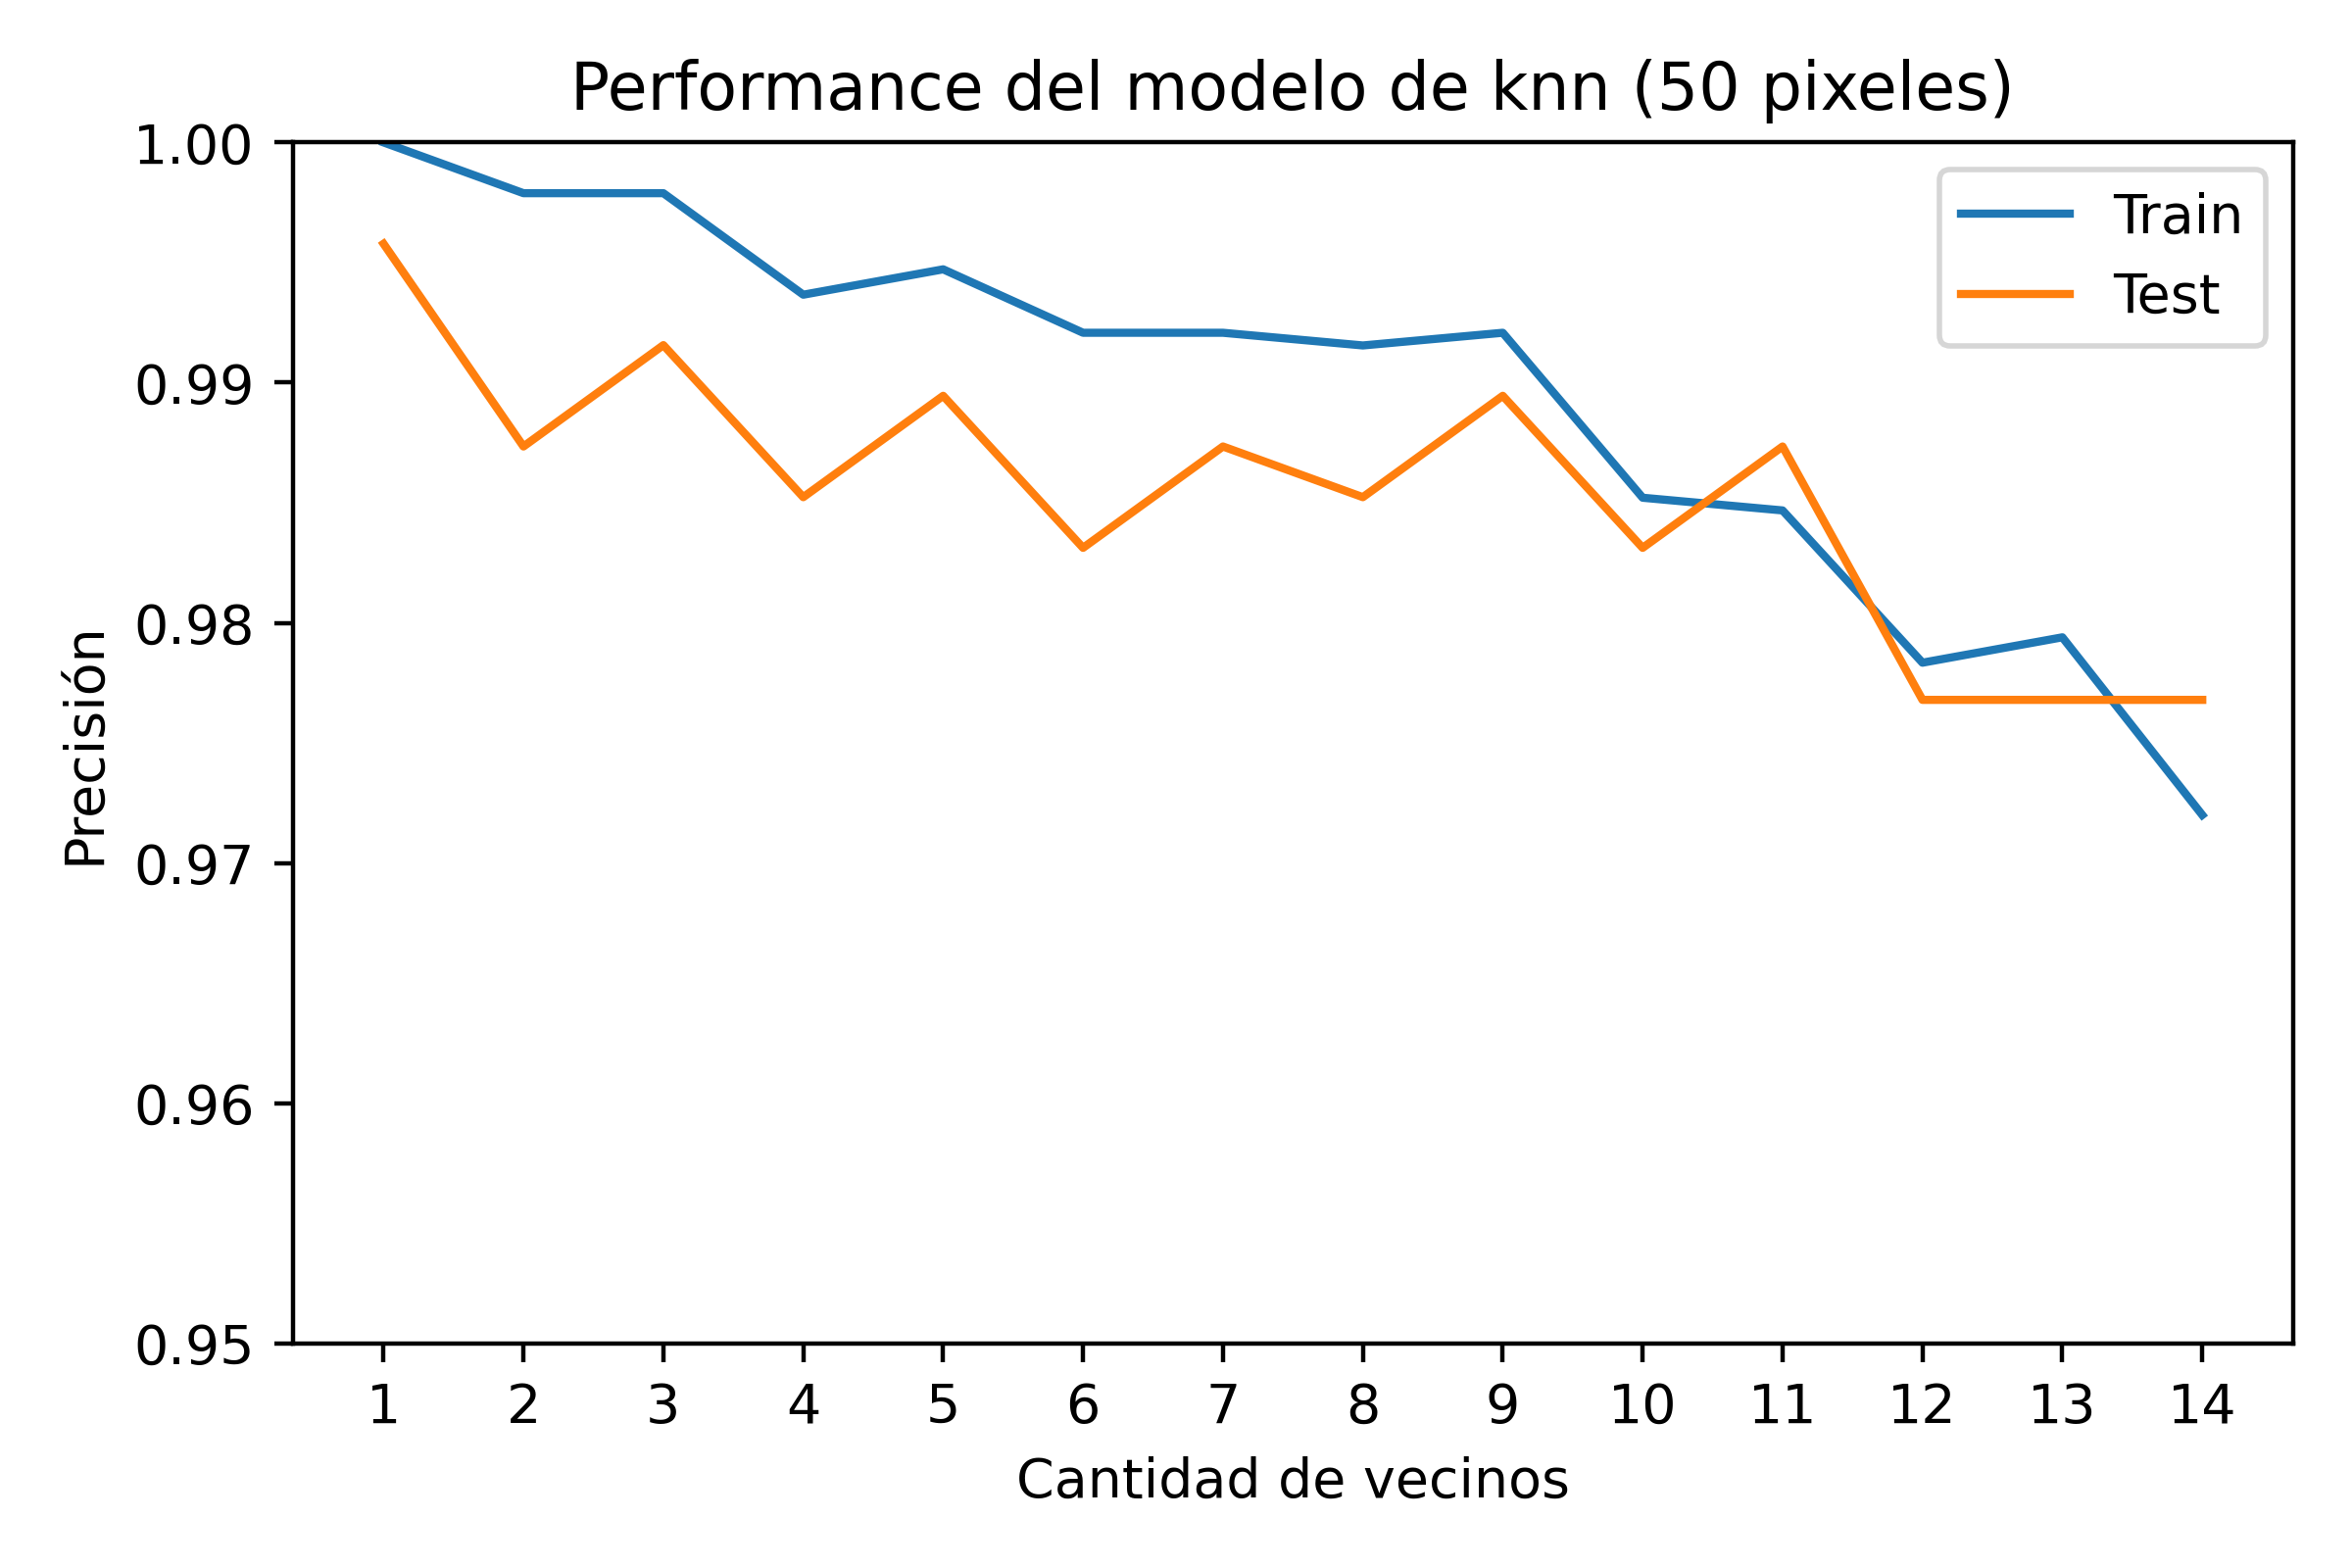
\includegraphics[width=0.9\linewidth]{Imagenes/50pixeles.png} 
		\caption{50 pixeles en una zona no tan significativa}
		\label{fig:subfig1}
	\end{subfigure}
	\begin{subfigure}{0.5\textwidth}
		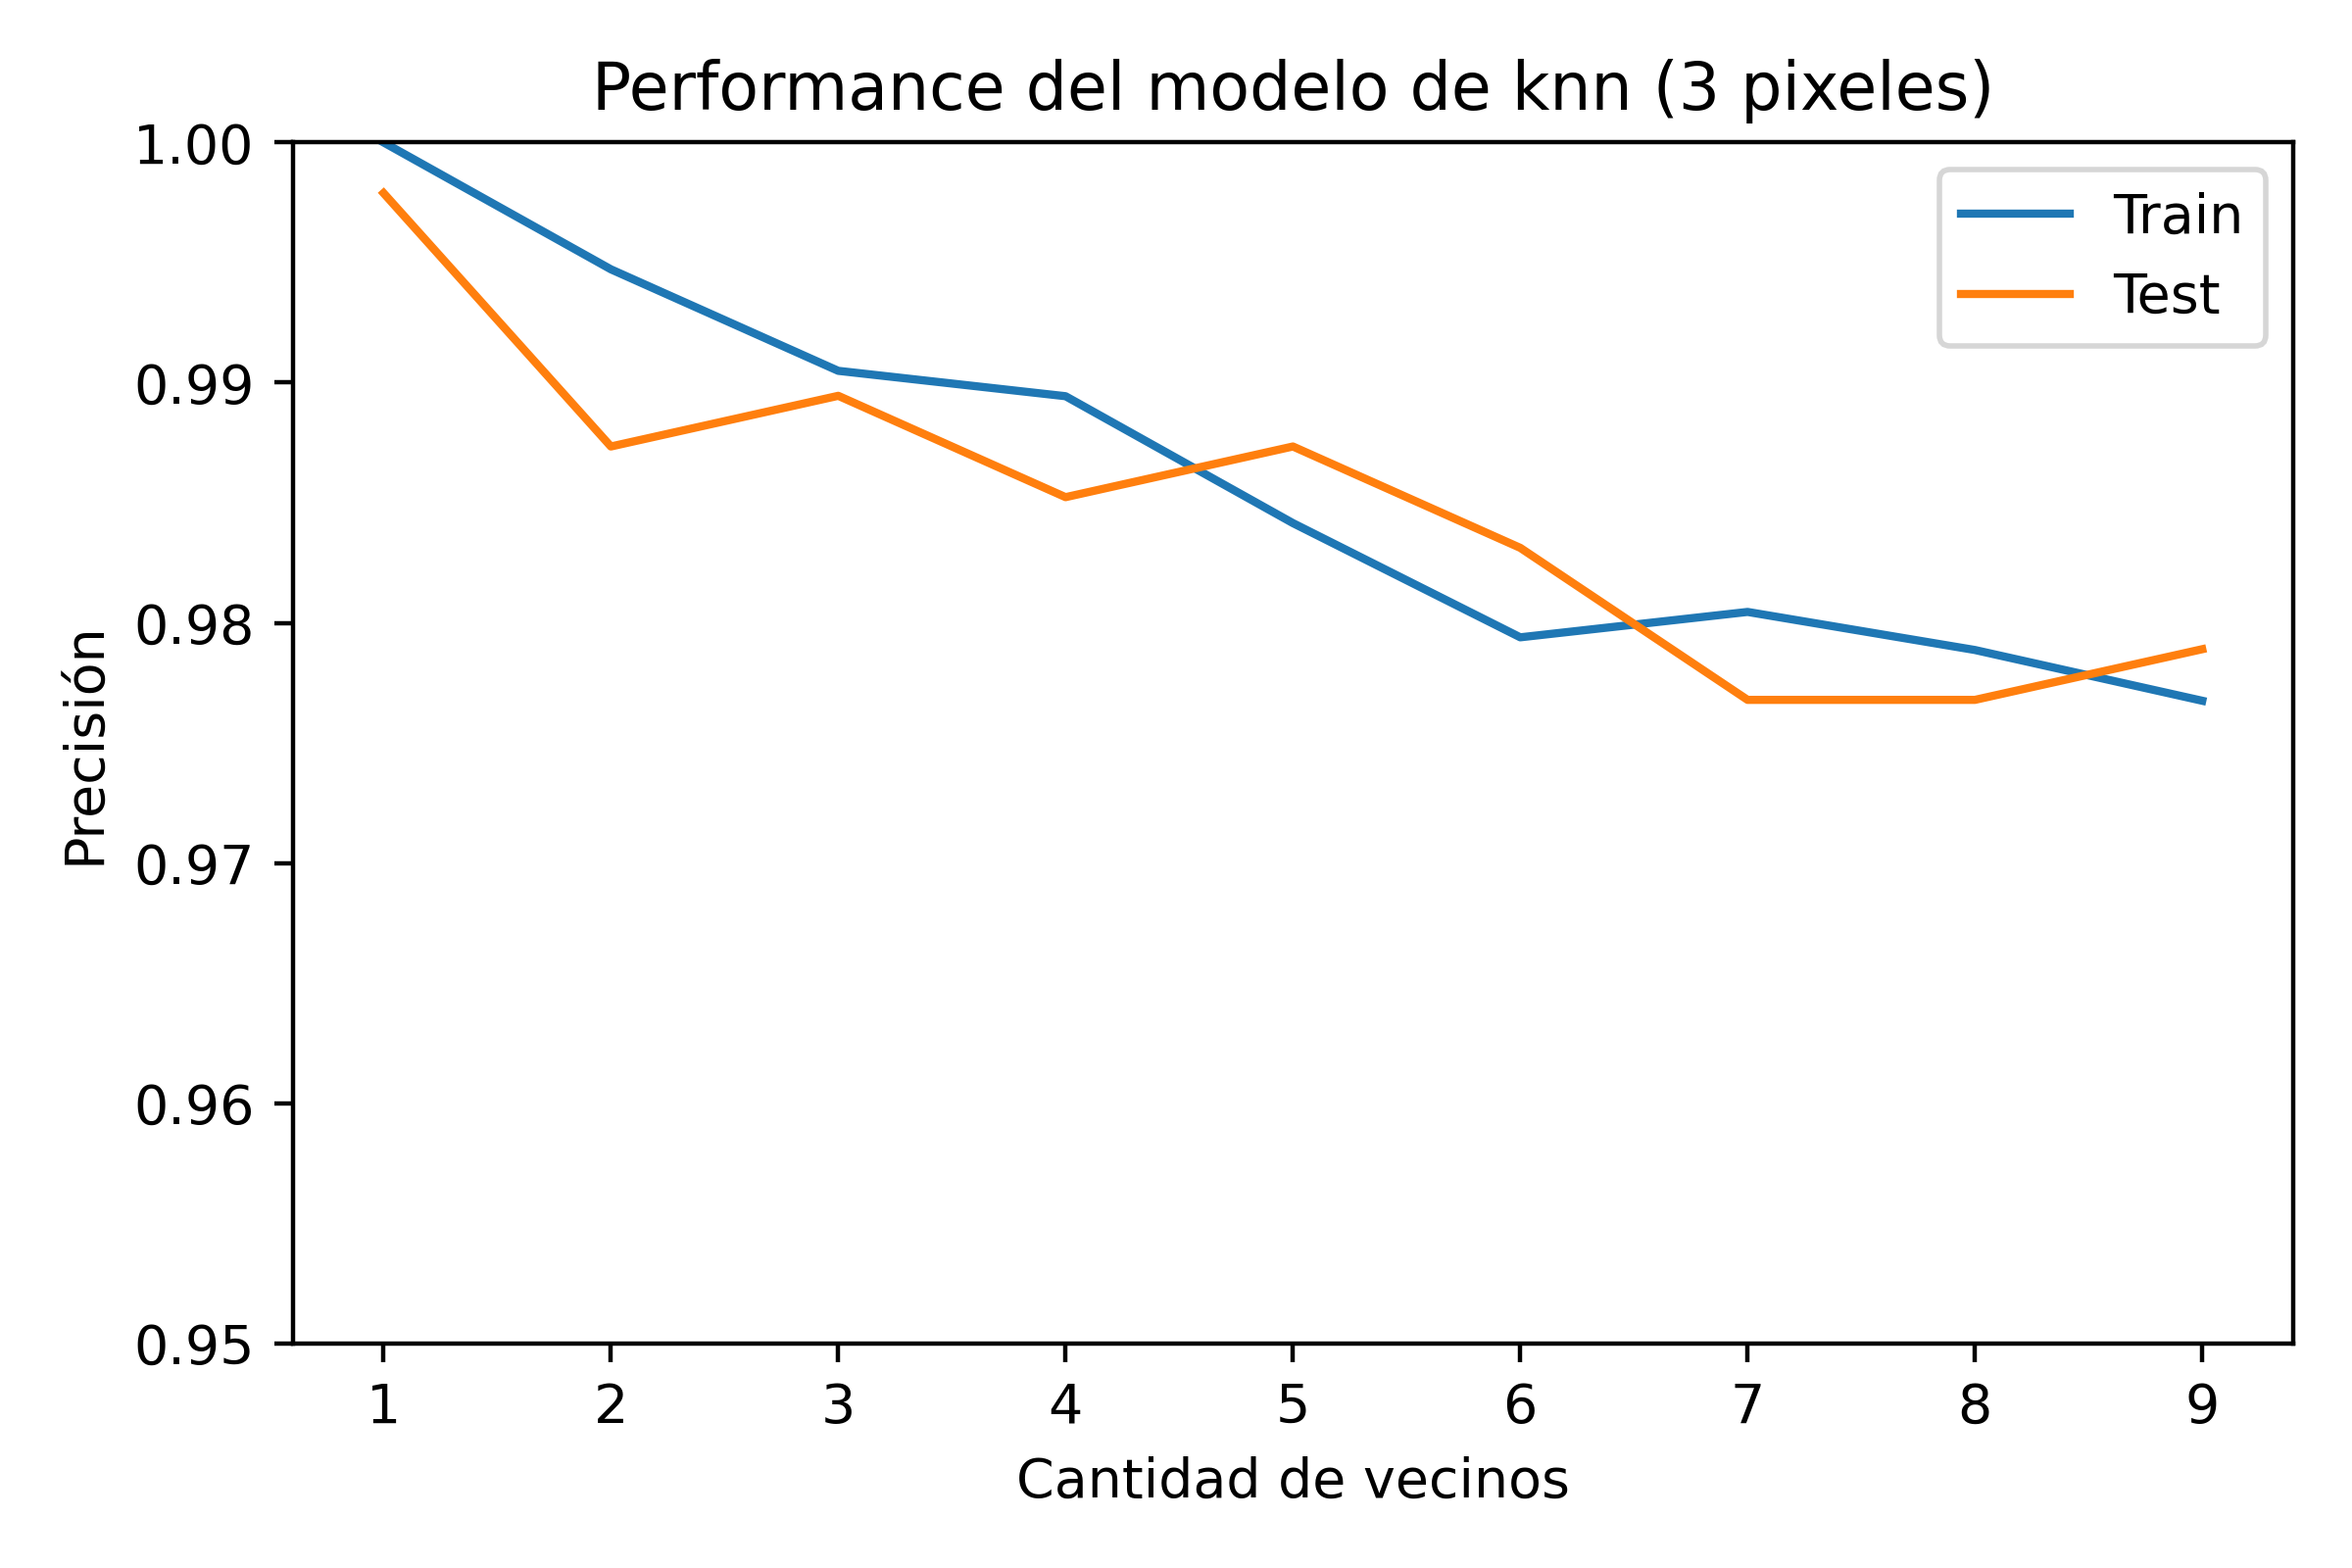
\includegraphics[width=0.9\linewidth]{Imagenes/3pixeles.png}
		\caption{Los 3 pixeles mas significativos}
		\label{fig:subfig2}
	\end{subfigure}
	% OJO: el caption siempre va antes del label
	\label{fig:subfigs}
\end{figure}

Notemos que, a diferencia de lo que marca la intuición, la mejor cantidad de vecinos es 1 en ambos casos. Por otro lado, podemos notar que no es necesaria una gran cantidad de pixeles, sino que solamente con 3 pixeles que sean relevantes podemos tener un modelo con mas del 0.99 de precisión.

\newpage

\begin{figure}[ht!]
	\begin{subfigure}{0.5\textwidth}
		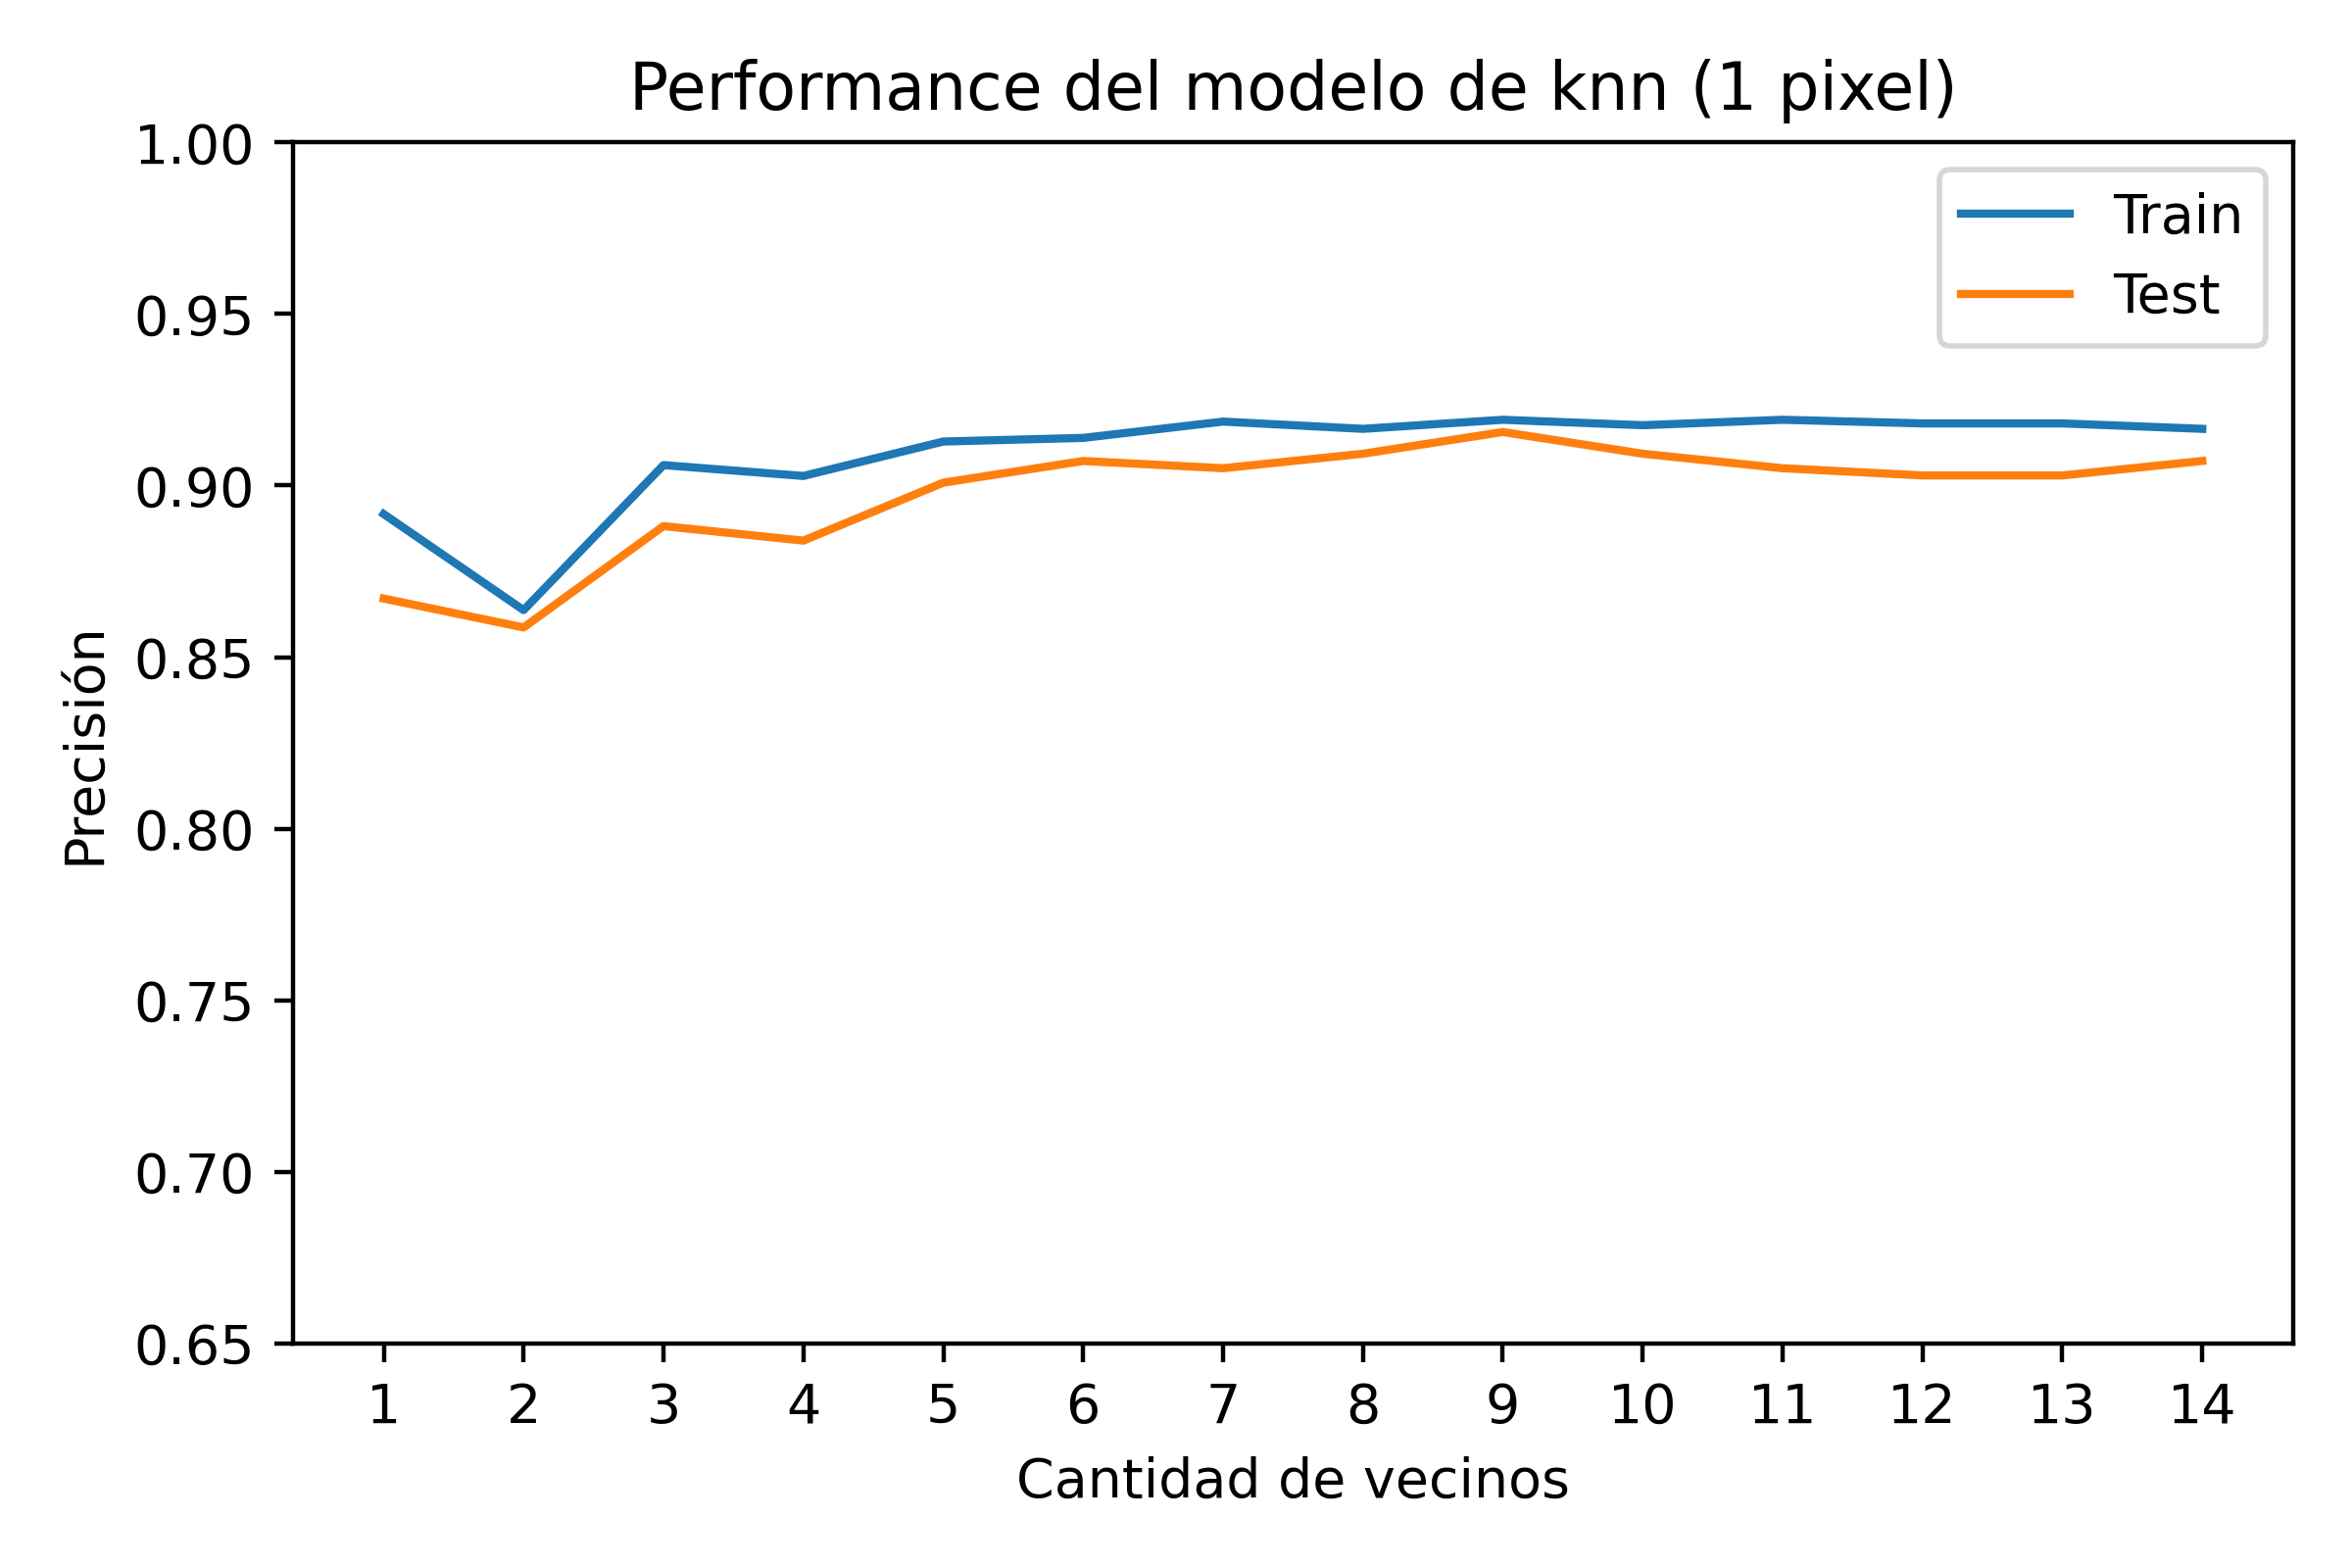
\includegraphics[width=0.9\linewidth]{imagenes/1pixelalto.png} 
		\caption{Pixeles de alta varianza}
		\label{fig:subfig1}
	\end{subfigure}
	\begin{subfigure}{0.5\textwidth}
		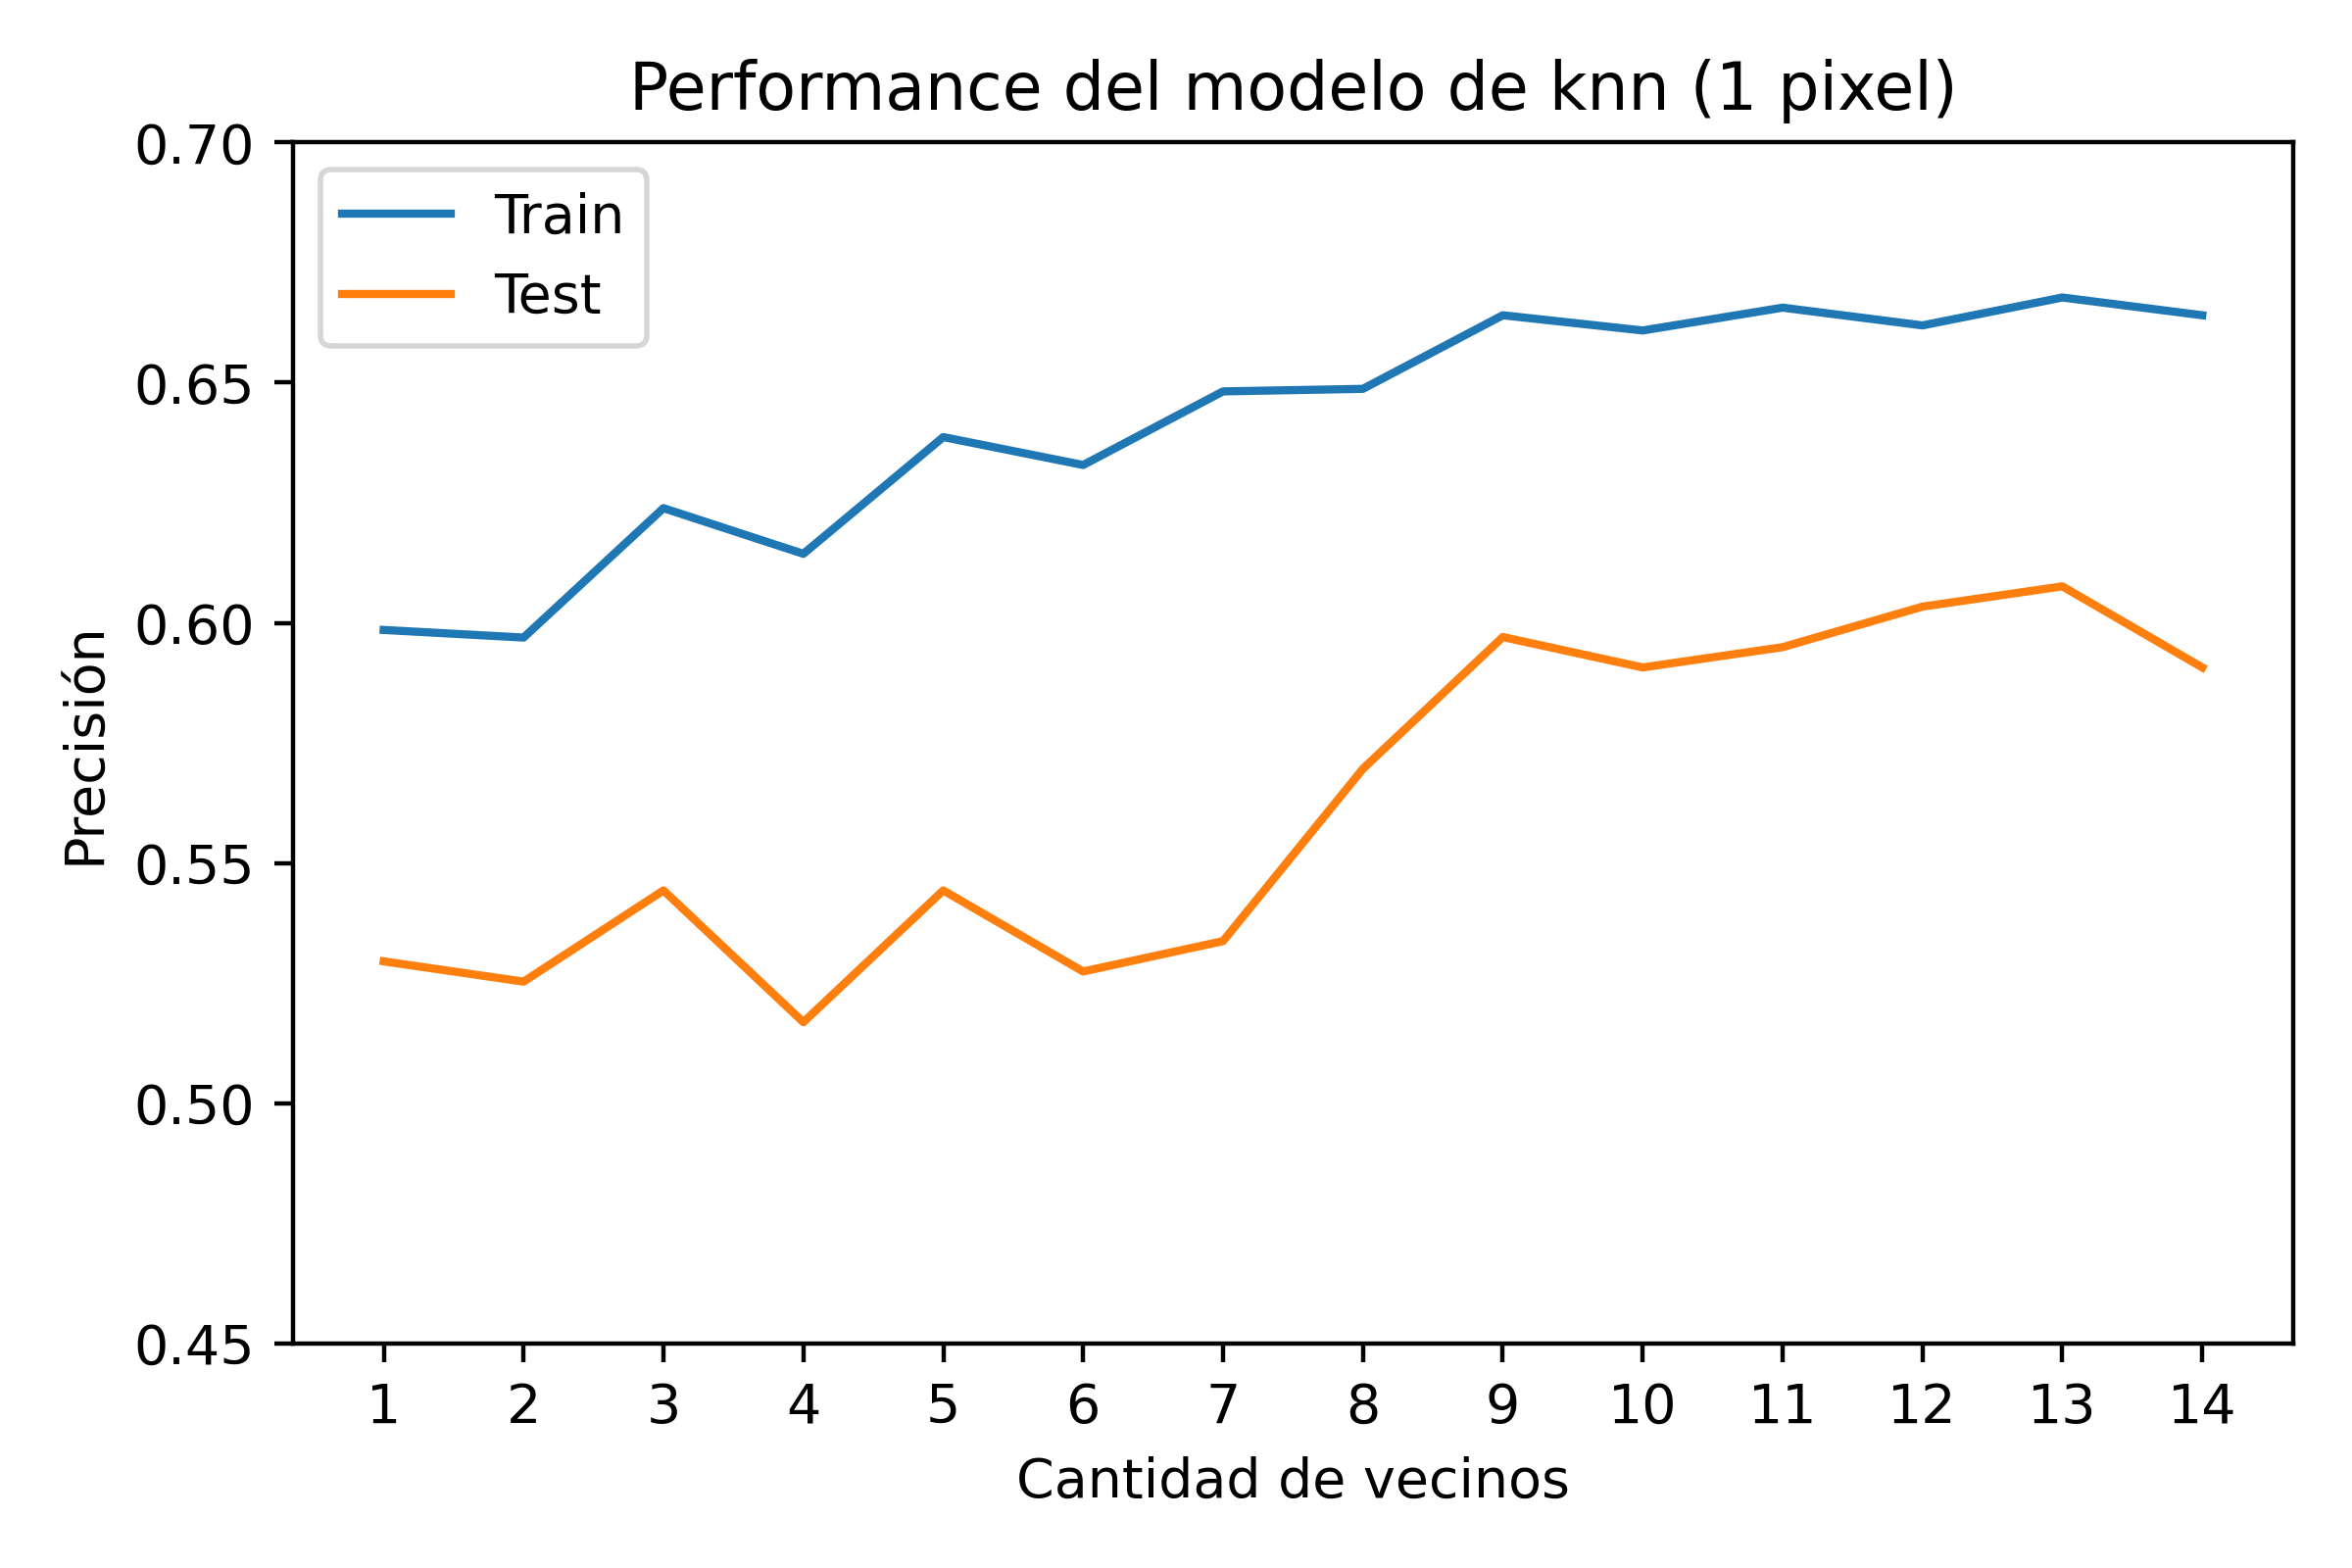
\includegraphics[width=0.9\linewidth]{Imagenes/1pixelbajo.png}
		\caption{Pixeles de baja varianza}
		\label{fig:subfig2}
	\end{subfigure}
	% OJO: el caption siempre va antes del label
	\label{fig:subfigs}
\end{figure}


Sin embargo, hay un caso que escapa a la regla. Encontramos que cuando tenemos solo un pixel. Sin importar si este es significativo o no, la performance del modelo tiende a aumentar a medida que el numero de vecinos es mayor. En este caso, a partir de los gráficos, pareciera ser que k = 9 sería un buen número.

\vspace{0.05cm}

Cerrando esta sección, creo que podemos concluir que tomando los 3 pixeles de mayor varianza y k = 1, tenemos un excelente clasificador para distinguir entre la letra A y la letra L.


\section{Clasificador Multiclase}



\end{document}
